\documentclass{beamer}
%\documentclass[handout]{beamer}

%\usepackage{graphics}
\usepackage{graphicx}
\usepackage{amsmath,amssymb,amsthm}
%\usepackage{subfigure}

%% To make 4 per page
%\usepackage{pgfpages}
%\mode<handout>{\setbeamercolor{background canvas}{bg=white}}
%\pgfpagesuselayout{4 on 1}[letterpaper,landscape]%,border shrink=5mm]




\def\IC{\mathbb{C}}
\def\IF{\mathbb{F}}
\def\II{\mathbb{I}}
\def\IM{\mathbb{M}}
\def\IN{\mathbb{N}}
\def\IP{\mathbb{P}}
\def\IR{\mathbb{R}}
\def\IZ{\mathbb{Z}}

\def\ba{\mathbf{a}}
\def\bb{\mathbf{b}}
\def\bc{\mathbf{c}}
\def\be{\mathbf{e}}
\def\bh{\mathbf{h}}
\def\bi{\mathbf{i}}
\def\bj{\mathbf{j}}
\def\bk{\mathbf{k}}
\def\bn{\mathbf{n}}
\def\bp{\mathbf{p}}
\def\br{\mathbf{r}}
\def\bs{\mathbf{s}}
\def\bu{\mathbf{u}}
\def\bv{\mathbf{v}}
\def\bw{\mathbf{w}}
\def\bx{\mathbf{x}}
\def\by{\mathbf{y}}
\def\bz{\mathbf{z}}

\def\bB{\mathbf{B}}
\def\bD{\mathbf{D}}
\def\bF{\mathbf{F}}
\def\bG{\mathbf{G}}
\def\bN{\mathbf{N}}
\def\bR{\mathbf{R}}
\def\bS{\mathbf{S}}
\def\bT{\mathbf{T}}
\def\b0{\mathbf{0}}

\def\A{\mathcal{A}}
\def\B{\mathcal{B}}
\def\C{\mathcal{C}}
\def\D{\mathcal{D}}
\def\E{\mathcal{E}}
\def\F{\mathcal{F}}
\def\G{\mathcal{G}}
\def\I{\mathcal{I}}
\def\L{\mathcal{L}}
\def\M{\mathcal{M}}
\def\P{\mathcal{P}}
\def\R{\mathcal{R}}
\def\S{\mathcal{S}}
\def\T{\mathcal{T}}
\def\U{\mathcal{U}}
\def\V{\mathcal{V}}

\newcommand\range{\mathsf{range}}
\renewcommand\null{\mathsf{null}}
\newcommand\diag{\mathsf{diag}}
\newcommand\tr{\mathsf{tr}}
\renewcommand\det{\mathsf{det}}
\newcommand\sgn{\mathsf{sgn}}
\renewcommand\span{\mathsf{span}}
\newcommand\imply{$\Rightarrow$}
\def\restrictTo#1#2{\left.#1\right|_{#2}}

\newcommand{\parallelsum}{\mathbin{\!/\mkern-5mu/\!}}

\def\Im{\textrm{Im}\;}
\def\Re{\textrm{Re}\;}

\newtheorem{proposition}[theorem]{Proposition}
\newtheorem{property}[theorem]{Property}
\newtheorem{importantproperty}[theorem]{Property}
\newtheorem{importanttheorem}[theorem]{Theorem}
%\newtheorem{lemma}[theorem]{Lemma}



\setbeamertemplate{navigation symbols}{}
\setbeamertemplate{footline}
{%
	\quad\insertsection\hfill p. \insertpagenumber\quad\mbox{}\vskip2pt
}
\usecolortheme{orchid}
\setbeamertemplate{theorems}[numbered]


\AtBeginSection[]
{
	\begin{frame}[noframenumbering,plain]
	\tableofcontents[currentsection,currentsubsection]
\end{frame}
%\addtocounter{framenumber}{-1}
}

%%%%%%%%%%%
% To have links to parts in the outline
\makeatletter
\AtBeginPart{%
\addtocontents{toc}{\protect\beamer@partintoc{\the\c@part}{\beamer@partnameshort}{\the\c@page}}%
}
%% number, shortname, page.
\providecommand\beamer@partintoc[3]{%
\ifnum\c@tocdepth=-1\relax
% requesting onlyparts.
\makebox[6em]{Chapter #1:} \textcolor{green!30!blue}{\hyperlink{#2}{#2}}
\par
\fi
}
\define@key{beamertoc}{onlyparts}[]{%
\c@tocdepth=-1\relax
}
\makeatother%

\newcommand{\nameofthepart}{}
\newcommand{\nupart}[1]%
{   \part{#1}%
\renewcommand{\nameofthepart}{#1}%
\begin{frame}{#1}%\partpage 
\hypertarget{\nameofthepart}{}\tableofcontents%
\end{frame}
}



%%%%%%% 
%% Definitions in yellow boxes
\usepackage{etoolbox}
\setbeamercolor{block title}{use=structure,fg=structure.fg,bg=structure.fg!20!bg}
\setbeamercolor{block body}{parent=normal text,use=block title,bg=block title.bg!50!bg}

\BeforeBeginEnvironment{definition}{%
\setbeamercolor{block title}{fg=black,bg=yellow!50!white}
\setbeamercolor{block body}{fg=black, bg=yellow!30!white}
}
\AfterEndEnvironment{definition}{
\setbeamercolor{block title}{use=structure,fg=structure.fg,bg=structure.fg!20!bg}
\setbeamercolor{block body}{parent=normal text,use=block title,bg=block title.bg!50!bg, fg=black}
}
\BeforeBeginEnvironment{importanttheorem}{%
\setbeamercolor{block title}{fg=black,bg=red!50!white}
\setbeamercolor{block body}{fg=black, bg=red!30!white}
}
\AfterEndEnvironment{importanttheorem}{
\setbeamercolor{block title}{use=structure,fg=structure.fg,bg=structure.fg!20!bg}
\setbeamercolor{block body}{parent=normal text,use=block title,bg=block title.bg!50!bg, fg=black}
}
\BeforeBeginEnvironment{importantproperty}{%
\setbeamercolor{block title}{fg=black,bg=red!50!white}
\setbeamercolor{block body}{fg=black, bg=red!30!white}
}
\AfterEndEnvironment{importantproperty}{
\setbeamercolor{block title}{use=structure,fg=structure.fg,bg=structure.fg!20!bg}
\setbeamercolor{block body}{parent=normal text,use=block title,bg=block title.bg!50!bg, fg=black}
}









\begin{document}

\begin{frame}[noframenumbering,plain]{OUTLINE}
\tableofcontents[onlyparts]
\end{frame}


%%%%%%%%%%%%%%%%%%%%%
%%%%%%%%%%%%%%%%%%%%%
%%%%%%%%%%%%%%%%%%%%%
%%%%%%%%%%%%%%%%%%%%%
%%%%%%%%%%%%%%%%%%%%%
%%%%%%%%%%%%%%%%%%%%%
%%%%%%%%%%%%%%%%%%%%%
%%%%%%%%%%%%%%%%%%%%%
%%%%%%%%%%%%%%%%%%%%%
%%%%%%%%%%%%%%%%%%%%%
%%%%%%%%%%%%%%%%%%%%%
%%%%%%%%%%%%%%%%%%%%%
\nupart{Review (linear algebra and a few other things)}


\begin{frame}
In this course, we rely on notions you acquired in MATH 1210/1240/1300
\vfill
Here, we do a refresher of material in these courses. We also add (for some of you) a few things that will be handy and establish some terminology that we use throughout the course
\end{frame}

\section{Sets and logic}

\frame{\frametitle{Sets and elements}
	\begin{definition}[Set]
		A \textbf{set} $X$ is a collection of \textbf{elements}.
	\end{definition}
	We write $x\in X$ or $x\not\in X$ to indicate that the element $x$ belongs to
	the set $X$ or does not belong to the set $X$, respectively.
	\vfill
	\begin{definition}[Subset]
		Let $X$ be a set. The set $S$ is a \textbf{subset} of $X$, which is denoted
		$S\subset X$, if all its elements belong to $X$. We say $S$ is a \textbf{proper subset} of $X$ and write $S\subsetneq X$, if it is a subset of $X$ and not equal to $X$.
	\end{definition}
	
}


\frame{\frametitle{Quantifiers}
	A shorthand notation for ``for all elements $x$ belonging to $X$'' is $\forall x\in X$
	\vfill
	For example, if $X=\IR$, the field of real numbers, then $\forall x\in\IR$ means ``for all real numbers $x$''
	\vfill
	A shorthand notation for ``there exists an element $x$ in the set $X$'' is
	$\exists x\in X$
	\vfill
	$\forall$ and $\exists$ are \textbf{quantifiers}
}

\frame{\frametitle{Intersection and union of sets}
	Let $X$ and $Y$ be two sets
	\vfill
	\begin{definition}[Intersection]
		The intersection of $X$ and $Y$, $X\cap Y$, is the set of elements that belong
		to $X$ \textbf{and} to $Y$,
		\[
		X\cap Y=\{x:x\in X\textbf{ and } x\in Y\}
		\]
	\end{definition}
	\vfill
	\begin{definition}[Union]
		The union of $X$ and $Y$, $X\cup Y$, is the set of elements that belong
		to $X$ \textbf{or} to $Y$,
		\[
		X\cup Y=\{x:x\in X\textbf{ or } x\in Y\}
		\]
	\end{definition}
Note that in mathematics, or=and/or in common parlance
}

\frame{\frametitle{A teeny bit of logic}
	In a logical sense, a \textbf{proposition} is an assertion (or statement)
	whose truth value (true or false) can be asserted. For example, a theorem is a
	proposition that has been shown to be true. ``The sky is blue'' is also a
	proposition
	\vfill
	Let $A$ be a proposition. We generally write
	\[
	A
	\]
	to mean that $A$ is true, and 
	\[
	\mathbf{not}\ A
	\]
	to mean that $A$ is false.
	$\mathbf{not}\ A$ is the \textbf{contraposition} of $A$ (or $\mathbf{not}\ A$
	is the contraposite of $A$)
}

\frame{\frametitle{A teeny bit of logic (cont.)}
	Let $A,B$ be propositions. Then
	\begin{itemize}
		\item $A\Rightarrow B$ (read $A$ implies $B$) means that whenever $A$ is true,
		then so is $B$
		\item $A\Leftrightarrow B$, also denoted $A$ if and only if $B$ ($A$
		iff $B$ for short), means that $A\Rightarrow B$ \textbf{and} $B\Rightarrow A$
		We also say that $A$ and $B$ are equivalent.
	\end{itemize}
	\vfill
	Let $A$ and $B$ be propositions. Then
	\[
	(A\Rightarrow B)\Leftrightarrow(\mathbf{not}\ B\Rightarrow\mathbf{not}\ A)
	\]
}

\frame{\frametitle{Necessary or sufficient conditions}
	Suppose we want to establish whether a given statement $P$ is true, depending
	on the truth value of a statement $H$. Then we say that
	\begin{itemize}
		\item $H$ is a \textbf{necessary condition} if $P\Rightarrow H$ \\
		(It is necessary that $H$ be true for $P$ to be true; so whenever
		$P$ is true, so is $H$)
		\vfill
		\item $H$ is a \textbf{sufficient condition} if $H\Rightarrow P$ \\
		(It suffices for $H$ to be true for $P$ to also be true)
		\vfill
		\item $H$ is a \textbf{necessary and sufficient condition} if $H\Leftrightarrow
		P$, i.e., $H$ and $P$ are equivalent
	\end{itemize}
}

\frame{\frametitle{Playing with quantifiers}
	For the quantifiers $\forall$ (for all) and $\exists$ (there exists),
	\begin{center}
		$\exists$ is the contraposite of $\forall$
	\end{center}
	\vfill
	Therefore, for example, the contraposite of
	\[
	\forall x\in X,\exists y\in Y
	\]
	is
	\[
	\exists x\in X,\forall y\in Y
	\]
}

%%%%%%%%%%%%%%
%%%%%%%%%%%%%%
\section{Vectors and vector spaces}

\frame{
	A \textbf{vector} $a$ is an ordered $n$-tuple of real numbers. For
	$a_1,\ldots,a_n\in\IR$, 
	\[
	\ba=(a_1,\ldots,a_n)\in\IR^n
	\]
	is a vector. $a_1,\ldots,a_n$ are the \textbf{components} of $a$.
	Vectors are also denoted
	\[
	\ba=\langle a_1,\ldots,a_n\rangle
	\]
	If unambiguous, $a$. Otherwise, $\mathbf{a}$ or $\vec{a}$
}


\frame{\frametitle{Vector space}
	\begin{definition}[Vector space]
		A \textbf{vector space} over $\IR$ is a set $V$
		together with two binary operations, \textbf{vector addition}, denoted $+$,
		and \textbf{scalar multiplication}, that satisfy the relations:
		\begin{enumerate}
			\item $\forall\bu, \bv, \bw\in V$, $\bu+(\bv+\bw)=(\bu+\bv)+\bw$
			\item $\forall\bv, \bw\in V$, $\bv + \bw = \bw + \bv$
			\item $\exists\b0\in V$, the zero vector, such that $\bv +\b0
			= \bv$ for all $\bv\in V$
			\item $\forall\bv\in V$, there exists an element $\bw\in V$, the additive
			inverse of $\bv$, such that $\bv + \bw = \b0$
			\item $\forall\alpha\in\IR$ and $\forall \bv,\bw\in V$, $\alpha(\bv + \bw) = \alpha \bv +
			\alpha \bw$
			\item $\forall\alpha,\beta\in\IR$ and $\forall \bv\in V$, $(\alpha+\beta)\bv=
			\alpha \bv + \beta \bv$
			\item $\forall\alpha,\beta\in\IR$ and $\forall\bv\in V$, $\alpha (\beta\bv) =
			(\alpha\beta)\bv$
			\item $\forall\bv\in V$, $1\bv =\bv$
		\end{enumerate}
	\end{definition}
}

\frame{\frametitle{Norms}
	\begin{definition}[Norm]
		Let $V$ be a vector space over $\IR$, and $\bv\in V$ be a vector. The
		\textbf{norm} of $\bv$, denoted $\|\bv\|$, is a function from $V$ to $\IR_+$ that has the
		following properties:
		\begin{enumerate}
			\item For all $\bv\in V$, $\|\bv\|\geq 0$ with $\|\bv\|=0$ iff $\bv=\b0$
			\item For all $\alpha\in\IR$ and all $\bv\in V$, $\|\alpha \bv\|=|\alpha|\ \|\bv\|$
			\item For all $\bu,\bv\in V$, $\|\bu+\bv\|\leq\|\bu\|+\|\bv\|$
		\end{enumerate}
	\end{definition}
}

\frame{
	Let $V_n$ be a vector space (for example, $\IR^2$ or $\IR^3$).
	\vfill
	The \textbf{zero element} (or \textbf{zero vector}) is the vector $\b0=(0,\ldots,0)$.
	\vfill
	The \textbf{additive inverse} of $\ba=(a_1,\ldots,a_n)$ is $-\ba=(-a_1,\ldots,-a_n)$. 
	\vskip0.5cm
	For $\ba=(a_1,\ldots,a_n)\in V_n$, the length (or Euclidean norm) of $\ba$ is the
	\textbf{scalar}
	\[
	\|\ba\|=\sqrt{a_1^2+\cdots+a_n^2}
	\]
	We also write $|\ba|$.
	\vfill
	To \textbf{normalize} the vector $\ba$ consists in considering $\tilde\ba=\ba/\|\ba\|$, i.e., the vector in the same direction as $\ba$ that has unit length
}

\frame{\frametitle{Standard basis vectors}
	\begin{minipage}{0.49\textwidth}
		Vectors ${\bi}=(1,0,0)$, ${\bj}=(0,1,0)$ and ${\bk}=(0,0,1)$ are the \textbf{standard basis vectors} of $\IR^3$. A vector $\ba=(a_1,a_2,a_3)$ can then be written
		\[
		\ba=a_1{\bi}+a_2{\bj}+a_3{\bk}
		\]
	\end{minipage}
	\begin{minipage}{0.49\textwidth}
		\begin{center}
			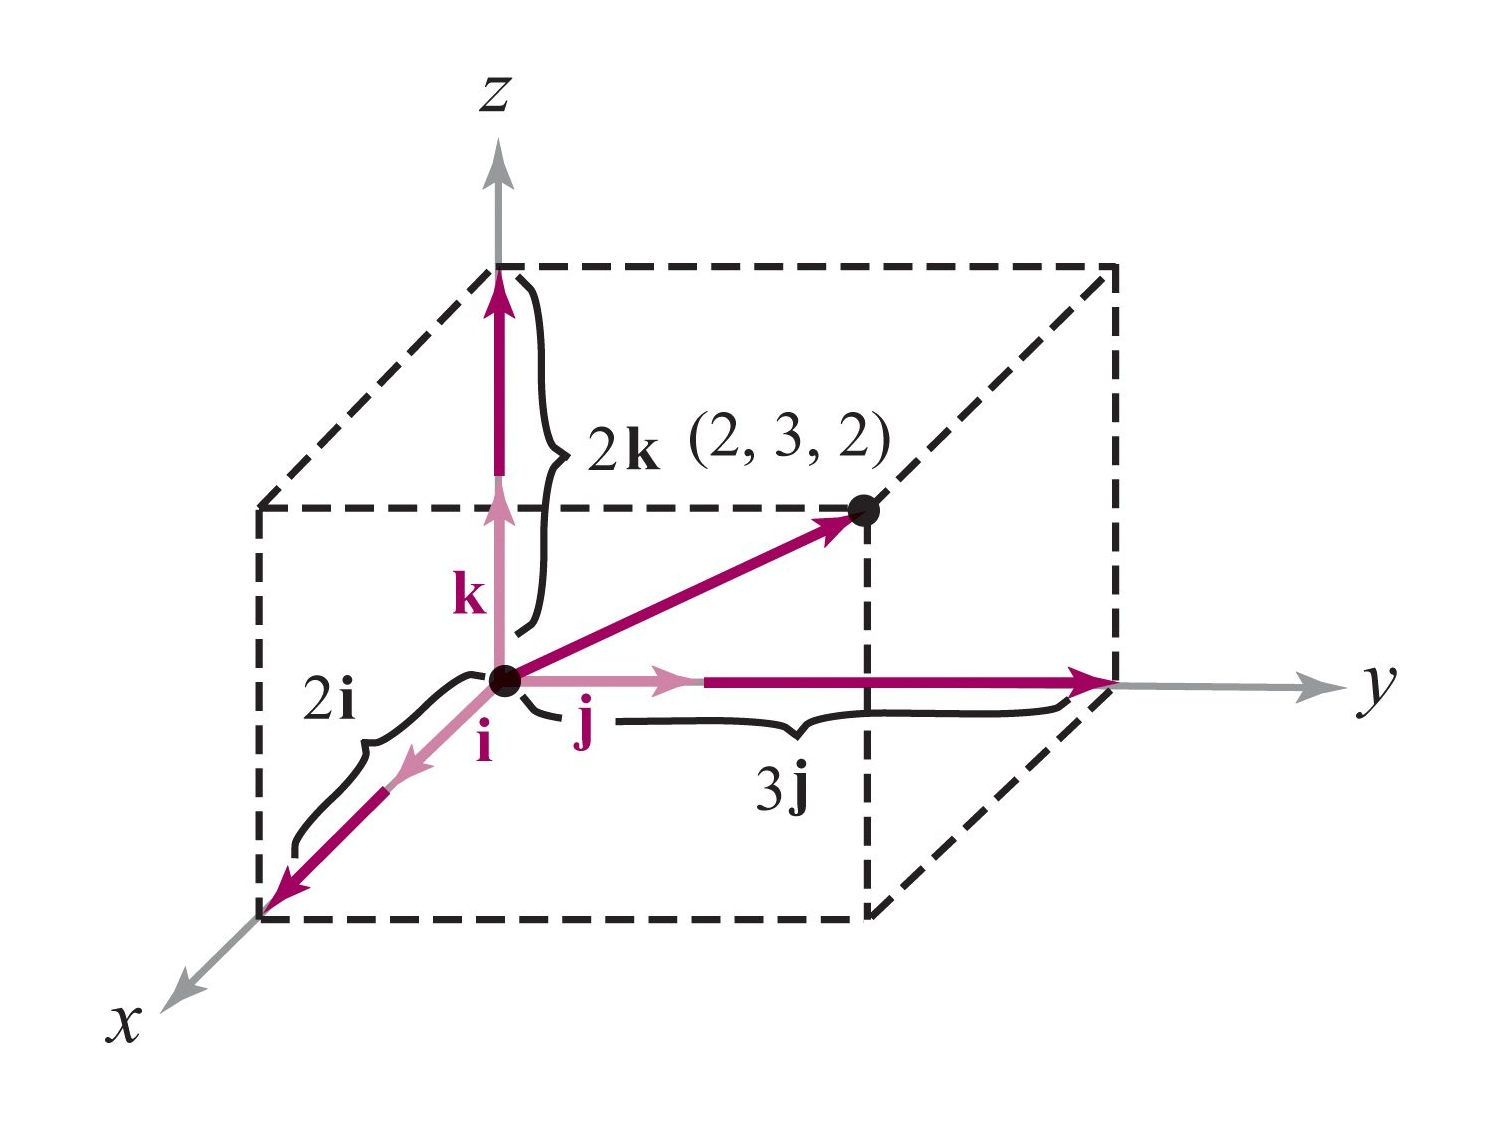
\includegraphics[width=1.15\textwidth]{FIGS_slides/vect_comb_lin_standard_basis_vectors}
		\end{center}
	\end{minipage}
	\vskip0.5cm
	For $V_n$ ($\IR^n$), the standard basis vectors are usually denoted $\be_1,\ldots,\be_n$, with 
	\[
	\be_k=(\underbrace{0,\ldots,0}_{k-1},1,\underbrace{0,\ldots,0}_{n-k+1})
	\]
}

%%%%%%%%%%%%%%
%%%%%%%%%%%%%%
\section{Inner product}
\frame{\frametitle{Inner product}
	\begin{definition}
		Let $\ba=(a_1,\ldots,a_n)\in V_n$, $\bb=(b_1,\ldots,b_n)\in V_n$. The \textbf{inner product} (or \textbf{dot product}) of $\ba$ and $\bb$ is the \textbf{scalar}
		\[
		\ba\bullet \bb=a_1b_1+\cdots+a_nb_n=\sum_{i=1}^n a_ib_i
		\]
	\end{definition}
}

\frame{\frametitle{Properties of the inner product}
	\begin{theorem}
		For $\ba,\bb,\bc\in V_n$ and $\alpha\in\IR$,
		\begin{itemize}
			\item $\ba\bullet\ba=\|\ba\|^2$ \hfill (so $\ba\bullet \ba\geq 0$, with $\ba\bullet \ba=0$ iff $\ba=\b0$)
			\item $\ba\bullet \bb=\bb\bullet \ba$ \hfill ($\bullet$ is commutative)
			\item $\ba\bullet(\bb+\bc)=\ba\bullet \bb+\ba\bullet \bc$ \hfill ($\bullet$ distributive over $+$)
			\item $(\alpha \ba)\bullet \bb=\alpha(\ba\bullet \bb)=\ba\bullet(\alpha \bb)$
			\item $\b0\bullet \ba=0$
		\end{itemize}
	\end{theorem}
}

\frame{\frametitle{Some results stemming from the inner product}
	\begin{theorem}
		If $\theta$ is the angle between the vectors $\ba$ and $\bb$, then
		\[
		\ba\bullet \bb=\|\ba\|\;\|\bb\|\;\cos\theta
		\]
	\end{theorem}
	\begin{corollary}[Cauchy-Schwarz inequality]
		For any two vectors $\ba$ and $\bb$, we have
		\[
		|\ba\bullet \bb|\leq \|\ba\|\;\|\bb\|
		\]
		with equality if and only if $\ba$ is a scalar multiple of $\bb$, or one of them is $\b0$.
	\end{corollary}
	\begin{theorem}
		$\ba$ and $\bb$ are orthogonal if and only if $\ba\bullet \bb=0$.
	\end{theorem}
}

\frame{\frametitle{Scalar and vector projections}
	Scalar projection of $\bv$ onto $\ba$ (or component of $\bv$ along $\ba$):
	\[
	\textrm{comp}_\ba\bv=\frac{\ba\bullet \bv}{\|\ba\|}
	\]
	\begin{minipage}{0.59\textwidth}
		Vector (or orthogonal) projection of $\bv$ onto $\ba$:
		\[
		\textrm{proj}_\ba\bv=\left(\frac{\ba\bullet \bv}{\|\ba\|}\right)\frac{\ba}{\|\ba\|}
		=\frac{\ba\bullet \bv}{\|\ba\|^2}\ba
		\]
	\end{minipage}
	\begin{minipage}{0.39\textwidth}
		\begin{center}
			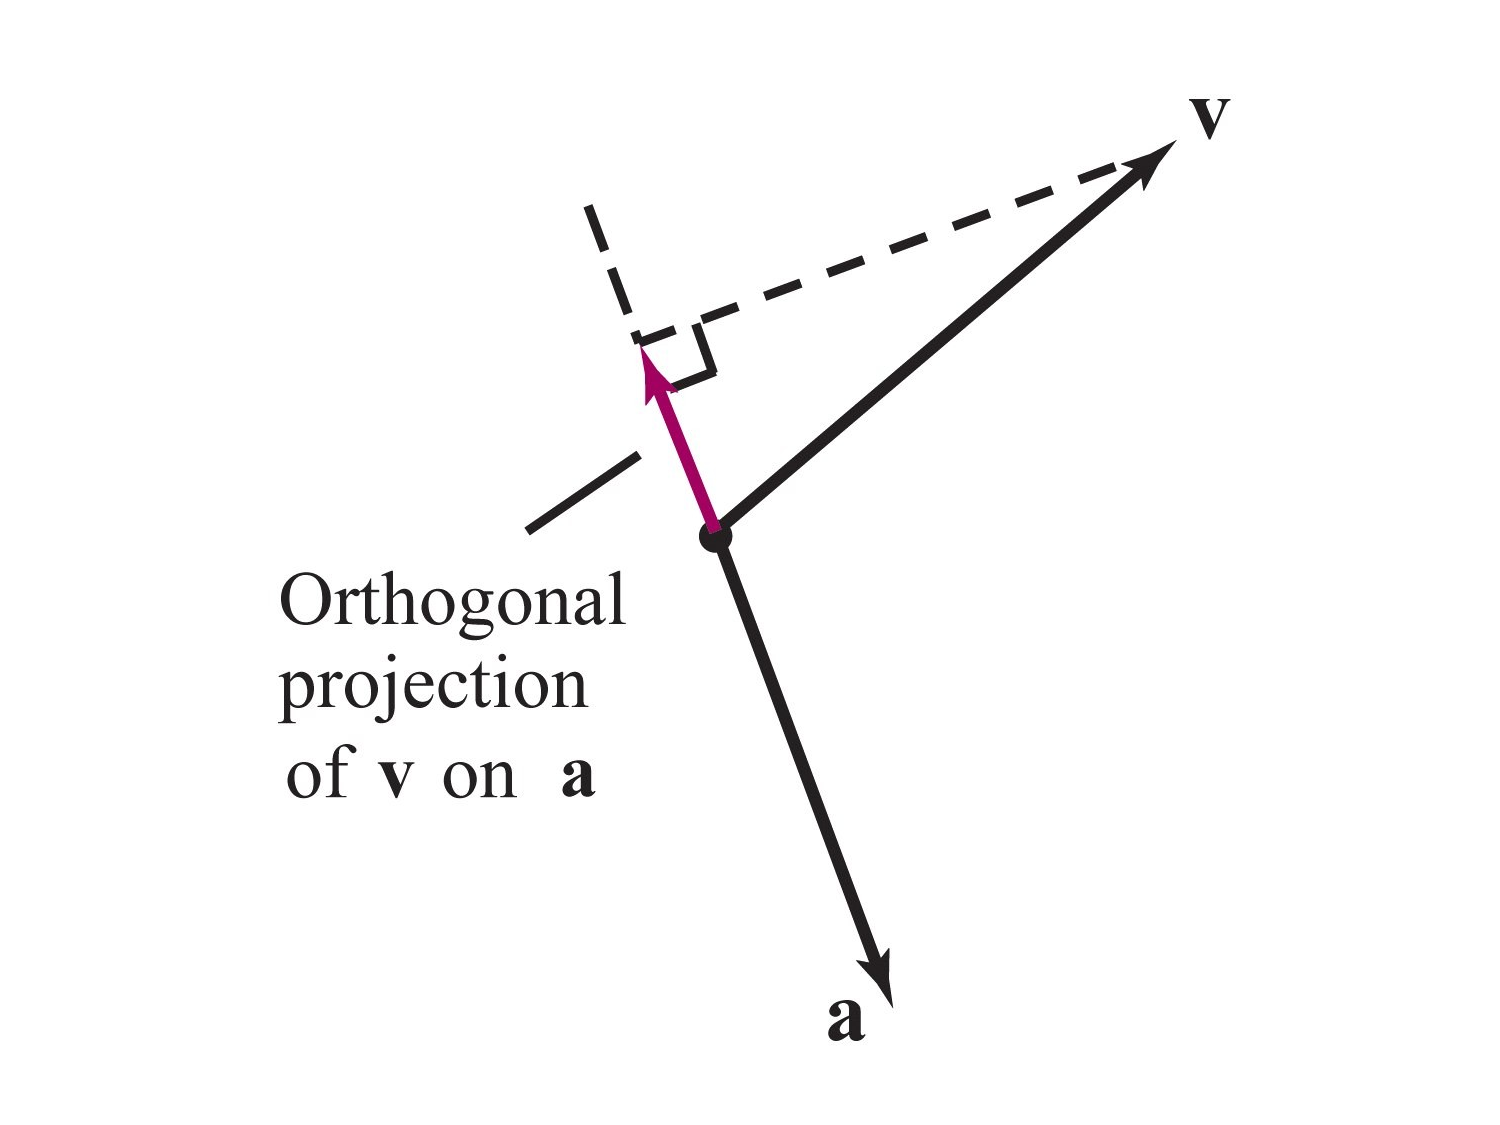
\includegraphics[width=1.1\textwidth]{FIGS_slides/proj_v_onto_a}
		\end{center}
	\end{minipage}
}


%%%%%%%%%%%%%%%%%%%%%
%%%%%%%%%%%%%%%%%%%%%
%%%%%%%%%%%%%%%%%%%%%
%%%%%%%%%%%%%%%%%%%%%
%%%%%%%%%%%%%%%%%%%%%
%%%%%%%%%%%%%%%%%%%%%
\section{Linear systems and matrices}


\begin{frame}{Linear systems}
\begin{definition}[Linear system]
A \textbf{linear system} of $m$ equations in $n$ unknowns takes the form
\begin{equation}\label{sys:linear_system}
\begin{matrix}
a_{11}x_1 &+& a_{12}x_2 &+& \cdots &+& a_{1n}x_n &=& b_1 \\
a_{21}x_1 &+& a_{22}x_2 &+& \cdots &+& a_{2n}x_n &=& b_2 \\
\vdots && \vdots && \vdots && \vdots && \vdots \\
a_{m1}x_1 &+& a_{m2}x_2 &+& \cdots &+& a_{mn}x_n &=& b_n
\end{matrix}
\end{equation}
\end{definition}
The $a_{ij}$, $x_j$ and $b_j$ could be in $\IR$ or $\IC$, although here we typically assume they are in $\IR$
\end{frame}

\begin{frame}
The aim is to find $x_1,x_2,\ldots,x_n$ that satisfy all equations simultaneously
\vfill
\begin{importanttheorem}[Nature of solutions to a linear system]
\label{th:nature_solutions_linear_system}
A linear system can have
\begin{itemize}
	\item no solution
	\item a unique solution
	\item infinitely many solutions
\end{itemize}
\end{importanttheorem}
\end{frame}


\begin{frame}{Matrices and linear systems}
Writing
$$
A=
\begin{pmatrix}
a_{11} & a_{12} & \cdots & a_{1n} \\
a_{21} & a_{22} & \cdots & a_{2n} \\
\vdots &\vdots & & \vdots \\
a_{m1} & a_{m2} & \cdots & a_{mn}
\end{pmatrix},\quad
x=
\begin{pmatrix}
x_1\\ x_2 \\ \vdots \\ x_n
\end{pmatrix}
\quad\textrm{and}\quad
b=
\begin{pmatrix}
b_1\\ b_2 \\ \vdots \\ b_n
\end{pmatrix}
$$
where $A$ is an $m\times n$ \textbf{matrix}, $x$ and $b$ are $n$ (column) \textbf{vectors} (or $n\times 1$ matrices), then the linear system in the previous slide takes the form
$$
Ax=b  
$$
\end{frame}



\begin{frame}{Notation for vectors}
We usually assume vectors are column vectors and thus write, e.g.,
$$
x=
\begin{pmatrix}
x_1\\ x_2 \\ \vdots \\ x_n
\end{pmatrix}
= (x_1,x_2,\ldots,x_n)^T
$$
Here, $^T$ is the \textbf{transpose operator} (more on this soon)
\end{frame}



\begin{frame}
Consider the system
\[
A\bx=\bb
\]
\vfill
If $\bb=\b0=(0,\ldots,0)^T$, the system is \textbf{homogeneous} and always has the solution $x=0$ and so the ``no solution'' option in Theorem~\ref{th:nature_solutions_linear_system} goes away
\end{frame}
%%%%%%%%%%%%%%%%%%%%%
%%%%%%%%%%%%%%%%%%%%%
%%%%%%%%%%%%%%%%%%%%%
%%%%%%%%%%%%%%%%%%%%%
%%%%%%%%%%%%%%%%%%%%%
%%%%%%%%%%%%%%%%%%%%%
\section{Complex numbers}

\begin{frame}{Complex numbers}
\begin{definition}[Complex numbers]
	A \textbf{complex number} is an ordered pair $(a,b)$, where $a,b\in\IR$. Usually written $a+ib$ or $a+bi$, where $i^2=-1$
	\vfill
	The set of all complex numbers is denoted $\IC$, 
	\[
	\IC=\{a+ib: a,b\in\IR\}
	\]
\end{definition}
\end{frame}

\begin{frame}
\begin{definition}[Addition and multiplication on $\IC$]
Letting $a+ib$ and $c+id\in\IC$, addition on $\IC$ is defined by
\[
(a+ib)+(c+id) = (a+c)+i(b+d)
\]
and multiplication on $\IC$ is defined by
\[
(a+ib)(c+id) = (ac-bd)+i(ad+bc)
\]
\end{definition}
\vfill
Latter equality easy to obtain using regular multiplication and $i^2=-1$
\end{frame}

\begin{frame}{Properties}
$\forall\alpha,\beta,\gamma\in\IC$,
\vfill
$\alpha+\beta=\beta+\alpha$ and $\alpha\beta=\beta\alpha$ \hfill[\textbf{commutativity}]
\vfill
$(\alpha+\beta)+\gamma=\alpha+(\beta+\gamma)$ and $(\alpha\beta)\gamma=\alpha(\beta\gamma)$ \hfill[\textbf{associativity}]
\vfill
$\gamma+0=\gamma$ and $\gamma 1=\gamma$ \hfill[\textbf{identities}]
\vfill
$\forall\alpha\in\IC$, $\exists\beta\in\IC$ unique s.t. $\alpha+\beta=0$ \hfill[\textbf{additive inverse}]
\vfill
$\forall \alpha\neq 0\in\IC$, $\exists\beta\in\IC$ unique s.t. $\alpha\beta=1$ \hfill[\textbf{multiplicative inverse}]
\vfill
$\gamma(\alpha+\beta)=\gamma\alpha+\gamma\beta$ \hfill[\textbf{distributivity}]
\end{frame}


\begin{frame}{Additive \& multiplicative inverse, subtraction, division}
\begin{definition}
Let $\alpha,\beta\in\IC$
\begin{itemize}
\item $-\alpha$ is the \textbf{additive inverse} of $\alpha$, i.e., the unique number in $\IC$ s.t. $\alpha+(-\alpha)=0$
\item \textbf{Subtraction} on $\IC$:
\[
\beta-\alpha=\beta+(-\alpha)
\]
\item For $\alpha\neq 0$, $1/\alpha$ is the \textbf{multiplicative inverse} of $\alpha$, i.e., the unique number in $\IC$ s.t.
\[
\alpha(1/\alpha)=1
\]
\item \textbf{Division} on $\IC$:
\[
\beta/\alpha=\beta(1/\alpha)
\]
\end{itemize}
\end{definition}
\end{frame}


\begin{frame}
\begin{definition}[Real and imaginary parts]
Let $z=a+ib$. Then $\Re z=a$ is \textbf{real part} and $\Im z=b$ is \textbf{imaginary part} of $z$
\end{definition}
\vfill
If ambiguous, write $\Re(z)$ and $\Im(z)$
\vfill
\begin{definition}[Conjugate and Modulus]
Let $z=a+ib\in\IC$. Then
\begin{itemize}
\item \textbf{Complex conjugate} of $z$ is
\[
\bar z = a-ib
\]
\item \textbf{Modulus} (or \textbf{absolute value}) of $z$ is
\[
|z|=\sqrt{a^2+b^2} \geq 0
\]
\end{itemize}
\end{definition}
\end{frame}

\begin{frame}{Properties of complex numbers}
Let $w,z\in\IC$, then
\begin{itemize}
\item $z+\bar z=2\Re z$
\item $z-\bar z=2i\Im z$
\item $z\bar z=|z|^2$
\item $\overline{w+z}=\bar w+\bar z$ and $\overline{wz}=\bar w\bar z$
\item $\overline{\bar z}=z$
\item $|\Re z|\leq |z|$ and $|\Im z|\leq |z|$
\item $|\bar z|=|z|$
\item $|wz|=|w|\;|z|$
\item $|w+z|\leq |w|+|z|$ \hfill[\textbf{triangle inequality}]
\end{itemize}
\end{frame}



\end{document}